\documentclass[a4paper]{report}
\usepackage{hyperref}
\usepackage{lastpage}
\usepackage{fancyhdr}
\usepackage{lineno}
\usepackage{listings}
\usepackage{german}
\usepackage[utf8]{inputenc}
\usepackage{amssymb}
\usepackage{graphicx}
\usepackage{tikz}
\usetikzlibrary{positioning,shapes.geometric}
\usepackage{pdflscape}
%\newcommand{\genasso}[2]{\begin{minipage}{0.7\textwidth}\begin{normalsize}\begin{flushleft}\textbf{{#1}}\end{flushleft}\end{normalsize}\vspace{-1cm}\begin{flushleft}\begin{small}{#2}\end{small}\end{flushleft}\end{minipage}\\\vspace{0.2cm}}
\pagenumbering{arabic}

\pagestyle{fancy} 
\newcommand{\frontmatter}{\clearpage \cfoot{\thepage\ }
\setcounter{page}{1}
\pagenumbering{Roman}}
\newcommand{\mainmatter}{\clearpage \lhead{\myAuth} \rhead{\myDate} \cfoot{} \rfoot{\thepage\ of \pageref{LastPage}}
\setcounter{page}{1}
\pagenumbering{arabic}}
\newcommand{\backmatter}{\clearpage \rfoot{\thepage\ }
\setcounter{page}{1}
\pagenumbering{alph}}


\newcommand{\makemytitlepage}{\begin{titlepage}
    \begin{center}
        \vspace*{0.8cm}
        
        \Huge
        \textbf{\myTitle}
        
        \vspace{1.5cm}
        
        \Large
        \myAuthor

        \vspace{1.8cm}

        %\begin{large}\textbf{Abstract:} \myAbstract \end{large}
        
\includegraphics[width=6cm]{./IM.jpg}  
        
        \vfill
        
        \huge
        \myAsso
        
        \vspace{1.3cm}
        
        \Large

        %\myDate
        \today
        
    \end{center}
\end{titlepage}}
\newcommand{\myAuth}{Team: *Iron Man*\\B. Pohl, K. Trogant, R. Enseleit, D. Hebecker}
\newcommand{\myAuthor}{Birgit Pohl 574353 (MO. 9-11)\\Kevin Trogant 572451 (Mo. 15-17)\\Ronja Enseleit 572404 (Mo. 15-17)\\Dustin Hebecker 571271 (MO. 9-11)}
\newcommand{\myAsso}{Group: *Iron Man*}
\newcommand{\myDate}{\today}

%%%%%%%%%%%%%%%%%%%%%%%%%%%%%%%%
%%Change Title !!!!!!!!!!!!!!!!!
%%%%%%%%%%%%%%%%%%%%%%%%%%%%%%%%
\newcommand{\myTitle}{Exercise Sheet 10}

\begin{document}
\frontmatter
\makemytitlepage
\mainmatter

%%%%%%%%%%%%%%%%%%%%%%%%%%%%%%%%%%%%%%%%%%%%%%%%%%%%%%%%%%
%% Only modify below here  and change myTitle!!!!!!!!!!!!!
%%%%%%%%%%%%%%%%%%%%%%%%%%%%%%%%%%%%%%%%%%%%%%%%%%%%%%%%%%
\section*{Aufgabe 1}

Aus der Vorlesung wird nicht ganz Klar ob der CFG den Code enthalten sollte oder nicht. Ich habe mich daher an der Formatierung auf dem Aufgabenblatt orientiert mit eienr erweiterung um return Values darzustellen. 

\subsection*{max}
  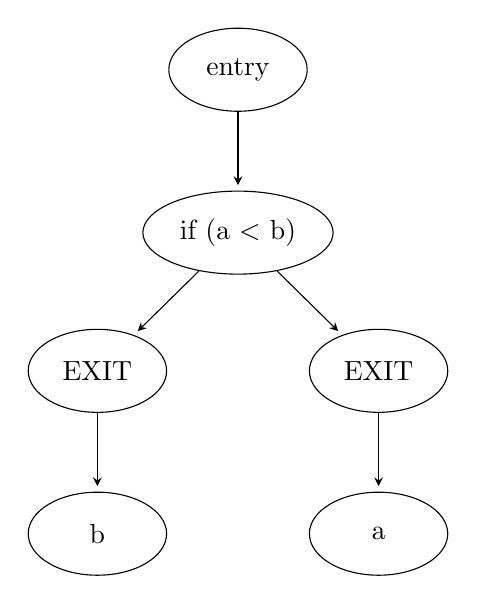
\begin{tikzpicture}[%
    ->,
    shorten >=2pt,
    >=stealth,
    node distance=1cm,
    noname/.style={%
      ellipse,
      minimum width=5em,
      minimum height=3em,
      draw
    }
  ]
    \node[noname] (1)                                             	{entry};
    \node[noname] (2) [below=of 1]                                	{if (a $<$ b)};
    \node[noname] (3) [node distance=1cm and 3mm,below left=of 2] 	{EXIT};
    \node[noname] (4) [node distance=1cm and 3mm,below right=of 2]	{EXIT};
    \node[noname] (5) [below=of 3]                                	{b};
    \node[noname] (6) [below=of 4]              			{a};

    \path (1) edge                   node {} (2)
          (2) edge                   node {} (3)
          (2) edge                   node {} (4)
          (3) edge                   node {} (5)
          (4) edge                   node {} (6);
  \end{tikzpicture}

  
  \subsection*{durchschnitt}
  \begin{tikzpicture}[%
    ->,
    shorten >=2pt,
    >=stealth,
    node distance=1cm,
    noname/.style={%
      ellipse,
      minimum width=5em,
      minimum height=3em,
      draw
    }
  ]
    \node[noname] (1)                                             	{entry};
    \node[noname] (2) [below=of 1]                                	{int ret=0, i=0};
    \node[noname] (4) [below=of 2]                                 	{if i$<$a.length};
    \node[noname] (5) [below left=of 4]                                	{ret+=a[i],i++};
    \node[noname] (6) [node distance=2cm,below right=of 4]		{Exit};
    \node[noname] (7) [below=of 6]              			{ret / a.length};
    
    \path (1) edge                   node {} (2)
          (2) edge                   node {} (4)
          (4) edge                   node {} (5)
          (5) edge                   node {} (4)
          (4) edge                   node {} (6)
          (6) edge		     node {} (7);
  \end{tikzpicture}
  
  
\begin{landscape}
\subsection*{nummer}
  \begin{tikzpicture}[%
    ->,
    shorten >=2pt,
    >=stealth,
    node distance=1cm,
    noname/.style={%
      ellipse,
      minimum width=5em,
      minimum height=3em,
      draw
    }
  ]
    \node[noname] (1)                                             	{entry};
    \node[noname] (2) [below=of 1]                                	{n};
    \node[noname] (3) [node distance=4cm and 5.5cm,below left=of 2] 				{Print ” Eins ! ”};
    \node[noname] (4) [right=of 3]                                 	{Print ” Zwei ! ”};
    \node[noname] (5) [right=of 4]                                {Print ” Drei ! ”};
    \node[noname] (6) [right=of 5]              			{Print ” Weder e i n s ,noch zwei ,noch d r e i. . . ” };
    \node[noname] (7) [below right=of 4]              			{Exit};
    
    \path (1) edge                   node {} (2)
          (2) edge                   node {} (3)
          (2) edge                   node {} (4)
          (2) edge                   node {} (5)
          (2) edge                   node {} (6)
          (3) edge 		     node {} (7)
          (4) edge 		     node {} (7)
          (5) edge 		     node {} (7)
          (6) edge 		     node {} (7);
 \end{tikzpicture}
\end{landscape}
  
  
\newpage
\section*{Aufgabe 2}
\begin{lstlisting}
void Funktion(bool a,bool b){
  int y=0;
  if(a){
    y+=2;
  }else{
    y++;
  }
  if(!b){
    y-=1;
  }
  return; //vermutlich "return y;" aber hier nicht ersichtlich
}
\end{lstlisting}

\newpage
\section*{Aufgabe 3}

\subsection*{1.}
Nein, es könnte sich z.B. um andere Variablentypen handeln. Die Max funktion könnte genauso eine min Funktion sein.
\subsection*{2.}
Nein, die exakte Implementierung kann anders sein und somit auch der Ablauf in der Maschiene. Ein Einfaches Beispiel ist:
\begin{lstlisting}
y+=x
\end{lstlisting}
und
\begin{lstlisting}
y=y+x
\end{lstlisting}
Der Code hat die selbe Bedeutung ist aber nicht identisch und wird bei mangelnder Compiler Optimierung auch anders ausgeführt. Siehe auch 3.1.
\subsection*{3.}
Ja.
\subsection*{4.}
Ja.


\end{document}
